\documentclass[twoside]{article}

\usepackage{lipsum}
\usepackage[sc]{mathpazo}
\usepackage[T1]{fontenc}
\linespread{1.05}
\usepackage{graphicx}
\usepackage{microtype}
\usepackage[hmarginratio=1:1,top=32mm,columnsep=20pt]{geometry}
\usepackage{multicol}
\usepackage[hang, small,labelfont=bf,up,textfont=it,up]{caption}
\usepackage{booktabs}
\usepackage{float}
\usepackage{hyperref}
\usepackage{lettrine}
\usepackage{paralist}
\usepackage{titlesec}
\renewcommand\thesection{\Roman{section}}
\renewcommand\thesubsection{\Roman{subsection}}
\titleformat{\section}[block]{\large\scshape\centering}{\thesection.}{1em}{}
\titleformat{\subsection}[block]{\large}{\thesubsection.}{1em}{}

\title{\vspace{-15mm}\fontsize{14pt}{10pt}\selectfont\textbf{Comparison of Traditional Personal Information Management Systems with a Newly Proposed Relational System}}
\author{
\large
\textsc{Vincent Wochnik}\\[2mm]
\normalsize Fontys University of Applied Sciences, Venlo \\
\normalsize \href{mailto:v.wochnik@student.fontys.nl}{v.wochnik@student.fontys.nl}
\vspace{-5mm}
}
\date{}

\begin{document}
\maketitle


\begin{multicols}{2}
\section*{Abstract}

\noindent Conventional personal information management systems such as diaries, to-do lists and analog notebooks are rather inconvenient for the management of information since information that is once written down cannot easily be combined with other information or moved to a different place. This newly proposed system treats data which can be text, speech or images as atoms which can then be connected with each other. This way, it becomes very easy to manage information once in the system.

This is where smartwatches come into play: A smartwatch is a terrible device for actually managing information but is excellent for the input of such. Information that has been entered in the system can then be managend using traditional devices such as smartphones or personal computers.

\section{Introduction}

Kind of research: Explanatory empirical research

Research Topic: Personal Information Management Systems

Research Objective: Establish a relationship between the currently available personal information management systems such as to-do lists as well as notebooks and a newly proposed relational way of storing information and consolidate the claim that the newly proposed model is more effective.

Research Question and Subquestions

Is a relational approach to personal information management systems more efficient?
Do people prefer the current way of information management?
Do people accept the newly proposed model?

\section{Criteria}


\subsection{Selection of Criteria}

The selection of criteria for the comparison of traditional and relational information management systems is done in a satisfactory manner to obtain a conclusion that can be relied upon for further investigation.

The list of criteria contains subjective as well as objective criteria. It has to be said, however, that all criteria is subjective in some way since two completely different solutions to one problem are compared by a set of criteria. Even the selection of those criteria is a subjective task done by the author of this paper.

\subsection{Objective Criteria}

\begin{itemize}
\item \textbf{Use of resources.} The amount of computational and storage resources the system requires.
\item \textbf{Complexity of data structure.} The complexity of the data structure required for operation of the system.
\end{itemize}

\subsection{Subjective Criteria}

\begin{itemize}
\item \textbf{Ease of use.} The easiness of use of the individual system. This criterion can be further divided:
\begin{itemize}
\item \textbf{Adding new information.}
\item \textbf{Finding existing information.}
\item \textbf{Reorganizing existing information.}
\end{itemize}
\item \textbf{Learning curve.} The subjective learning experience of the individual. This criterion can be further divided into multiple sub criteria:
\begin{itemize}
\item \textbf{Rate of adaptation.} The speed an individual can adapt to a newly introduced system that was previously unknown to that individual.
\item \textbf{Presence of obstacles.} The presence and rate of solving of obstacles in the learning of the newly introduced system.
\end{itemize}
\item \textbf{General appeal.} How much the system appeals to the individual subjectively.
\end{itemize}

\section{Analysis of Existing Systems}

\begin{table}[H]
\caption{Example table}
\centering
\begin{tabular}{llr}
\toprule
\multicolumn{2}{c}{Name} \\
\cmidrule(r){1-2}
First name & Last Name & Grade \\
\midrule
John & Doe & $7.5$ \\
Richard & Miles & $2$ \\
\bottomrule
\end{tabular}
\end{table}

\lipsum[5] % Dummy text

\begin{equation}
\label{eq:emc}
e = mc^2
\end{equation}

\lipsum[6] % Dummy text

\section{Application Proposal}

The proposal: An atomic data management system utilizing a smartwatch to take advantage of faster and more instantaneous data input.

\subsection{Atomic Data}

\begin{center}
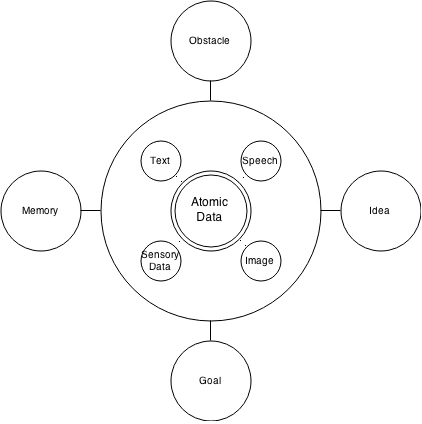
\includegraphics[width=0.9\linewidth]{00_resources/atomic_data.png}
\end{center}

Atomic data is in this case defined as small user-entered pieces of data which do not have to adhere to any standard.
On the right, a small illustration, the types of data the application supports can be seen.

\subsection{Data Input Methods}

\begin{center}
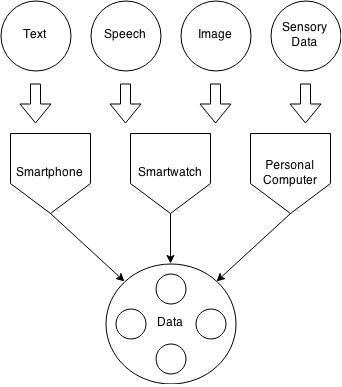
\includegraphics[width=0.9\linewidth]{00_resources/input_methods.png}
\end{center}

The data pieces can be inserted into the database utilizing the available input devices such as smartphones and smartwatches. Of course, a smartwatch can only capture little bits of information while a laptop can capture huge amounts. However, a smartwatch can be used instantly for capturing a piece of data while a laptop has to be prepared for capturing.

\subsection{Organization of Data}

Previously inserted atomic bits of data can be organized using a variety of models which are not all specified in this document. The more obvious ones are folders and labels as well as relationships between atomic data which can then be visualized as maps and radial relationship diagrams.

\subsubsection{Relationships}

\begin{center}
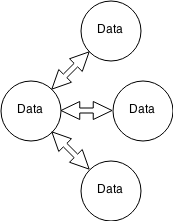
\includegraphics[width=0.5\linewidth]{00_resources/data_relationships.png}
\end{center}

Data can be organized in relationships where each relationship has two data atoms and a set of attributes such as the direction or the cardinality of the relationship. Relationships between data atoms can be displayed either on a map or on a radial graph showing only closest relations.

\subsubsection{Labels}

\begin{center}
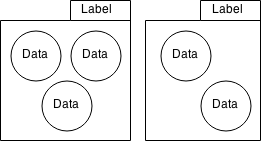
\includegraphics[width=0.5\linewidth]{00_resources/data_labels.png}
\end{center}

Data atoms can be grouped in labels or folders where each label optionally has attributes such as color.

\subsubsection{Timeline}

\begin{center}
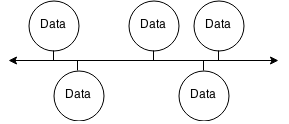
\includegraphics[width=0.5\linewidth]{00_resources/data_timeline.png}
\end{center}

Data atoms can be ordered by time either manually specified or by the creation time of the data atom itself.

\subsubsection{Matrix}

\begin{center}
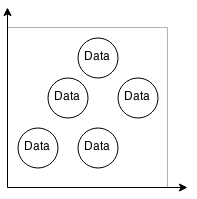
\includegraphics[width=0.5\linewidth]{00_resources/data_matrix.png}
\end{center}

Data atoms can be part of a two-dimensional matrix which can then be visualized.

\section{Conclusion}

blabla


\begin{thebibliography}{99}
\bibitem[Figueredo and Wolf, 2009]{Figueredo:2009dg}
Figueredo, A.~J. and Wolf, P. S.~A. (2009).
\newblock Assortative pairing and life history strategy - a cross-cultural
  study.
\newblock {\em Human Nature}, 20:317--330.

\end{thebibliography}
\end{multicols}
\end{document}
